\section{Simulation analysis}
\label{sec:simulation}
The simulation of the BPF, using the script given by the professor, will be analysed in this section.

\subsection{Frequency Response}
Right after simulating the circuit the frequency response of the same one both in $dB$ and phase are printed as bellow:

\begin{figure}[H] \centering
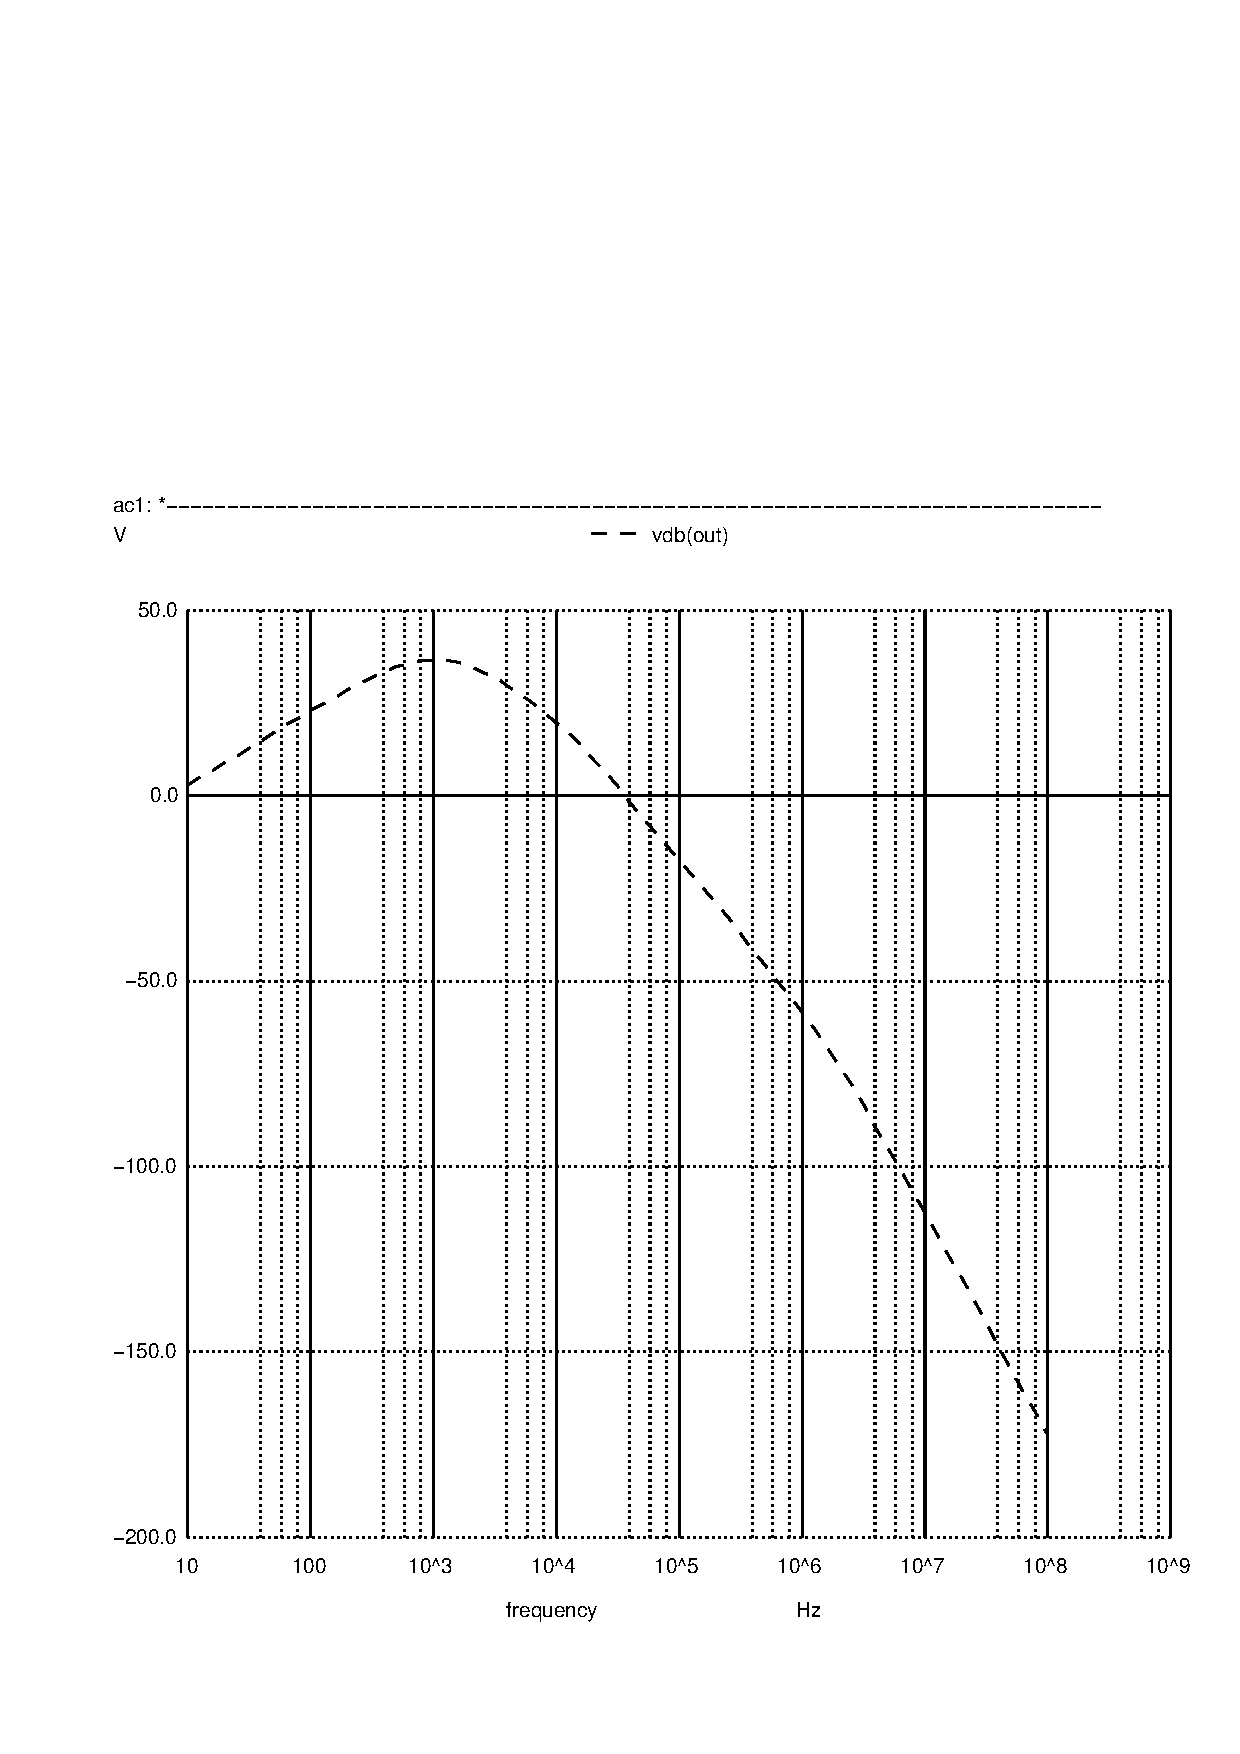
\includegraphics[width=0.7\linewidth]{../sim/vo1f.pdf}
\caption{Frequency Analysis in $dB$}
\label{fig:frequency1}
\end{figure}

\begin{figure}[H] \centering
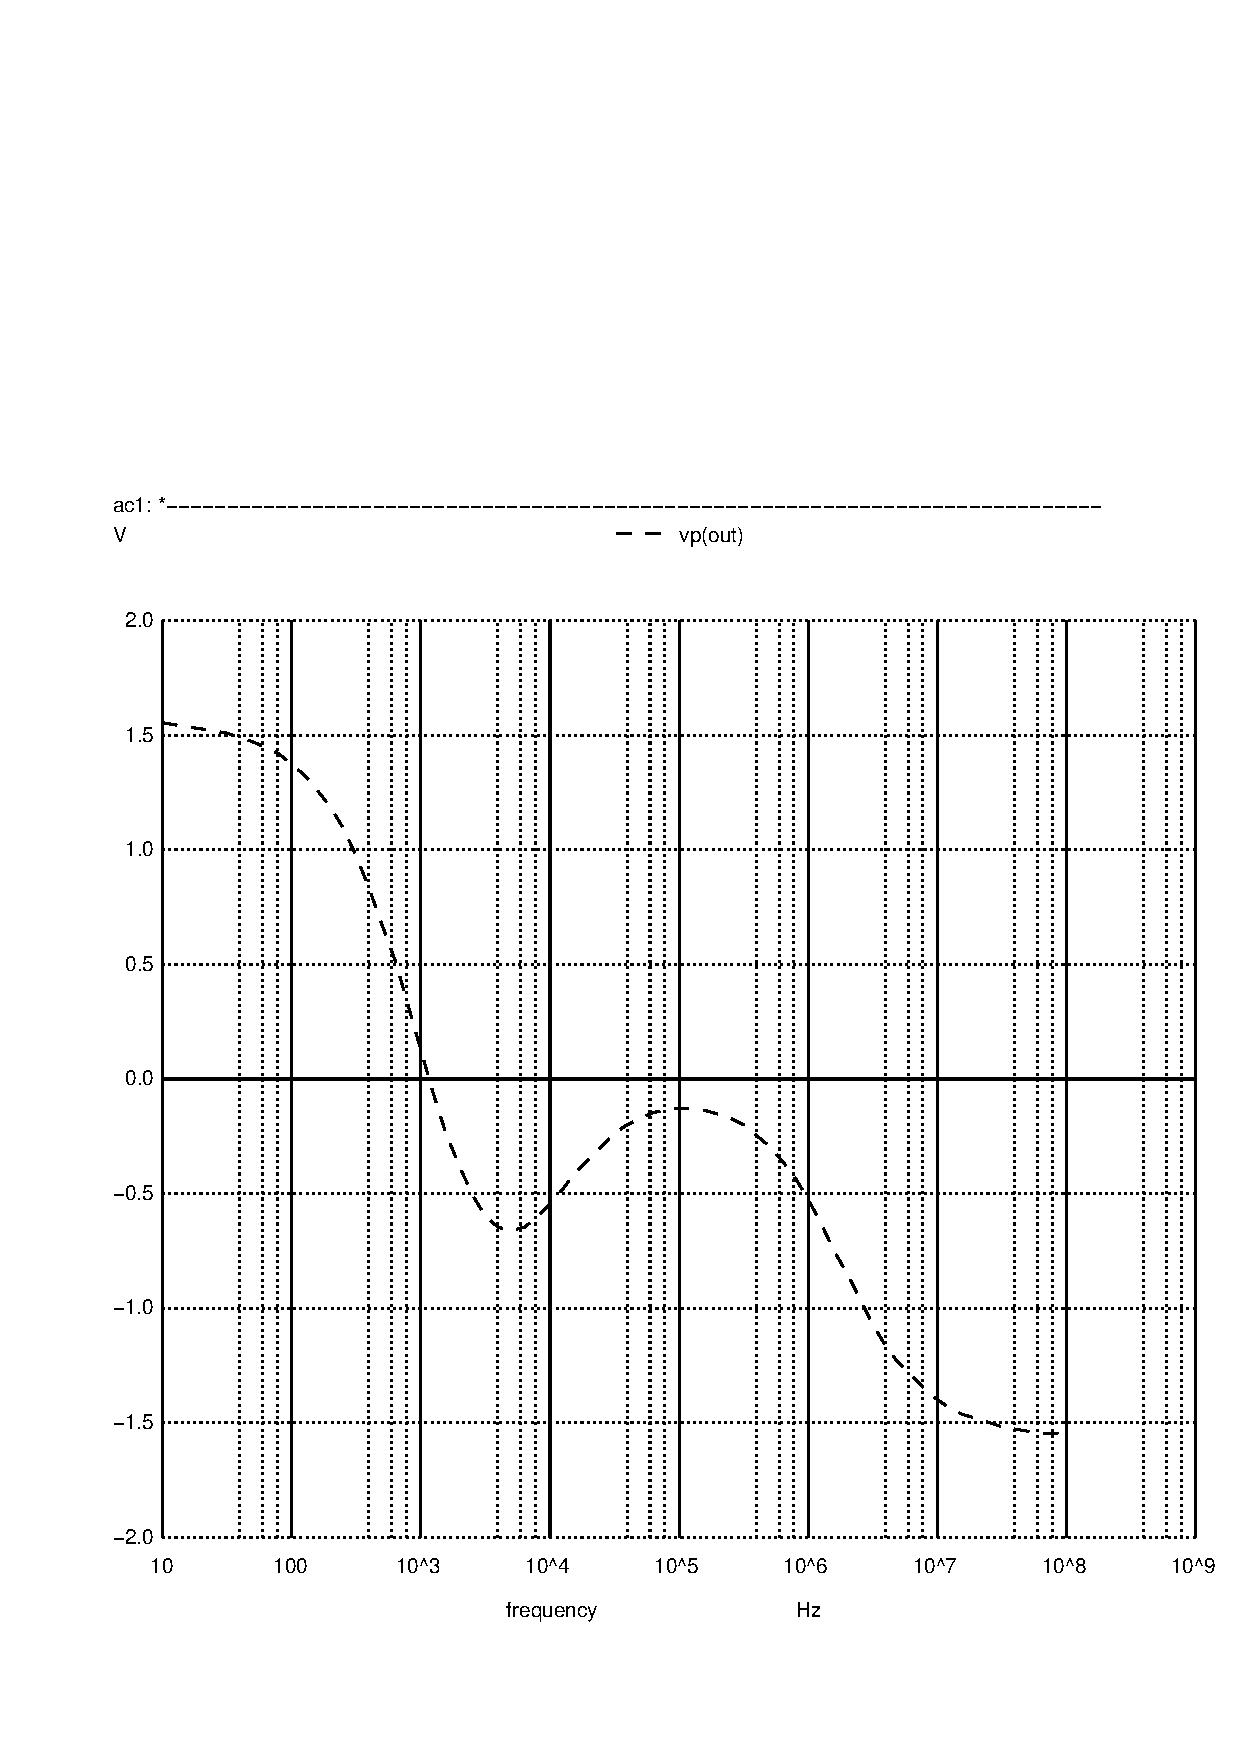
\includegraphics[width=0.7\linewidth]{../sim/vo1p.pdf}
\caption{Frequency Analysis - Phase}
\label{fig:frequency2}
\end{figure}

\subsection{Central Frequency in the Passband}
Our results were firstly analysed for the requested value in the laboratory assignment which was the central frequency in the passband. This was achieved by using the given equation by the professor: \par
\begin{equation}
    CentralFrequency = \sqrt{Lower_{cutoff} Upper_{cutoff}}
\end{equation}\par
In the images below the voltage is plotted. The lower and upper cutoff and central frequency values obtained are also in the table below:

\begin{figure}[H] \centering
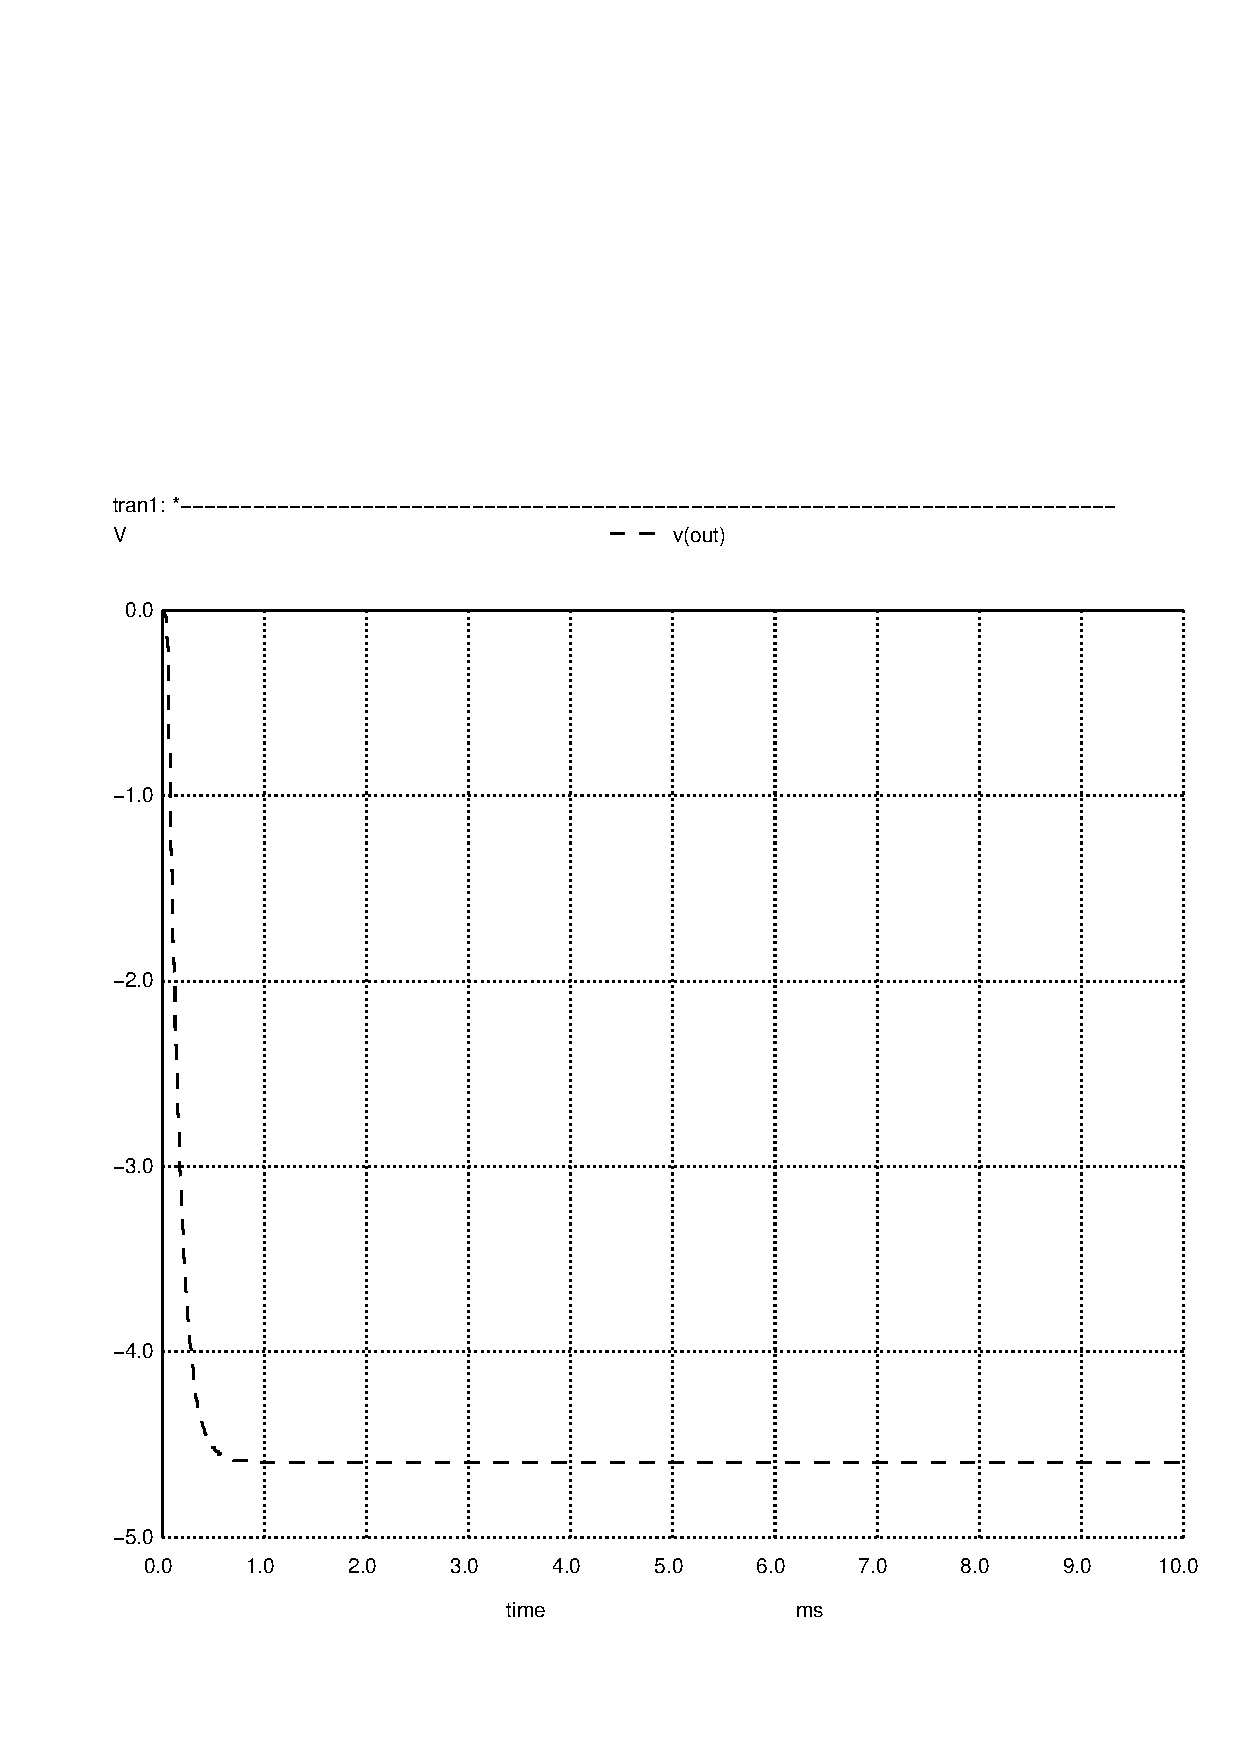
\includegraphics[width=0.7\linewidth]{../sim/vo1.pdf}
\caption{Output Voltage.}
\label{fig:output}
\end{figure}

\begin{table}[H]
  \centering
  \begin{tabular}{|l|r|}
    \hline    
    {\bf Name} & {\bf Value [$Hz$]} \\ \hline
    lower & 2.989834e+02\\ \hline
upper & 1.722537e+03\\ \hline
central & 7.176420e+02\\ \hline

  \end{tabular}
  \label{tab:central}
  \captionof{figure}{Central Frequency Gain}
\end{table}

\subsection{Output Voltage Gain}
In this section, the voltage gain in the frequency requested is calculated. \par
This voltage is the maximum of the difference of the out voltage in $dB$ and the in voltage in $dB$. \par
The value obtained is in the table below:

\begin{table}[H]
  \centering
  \begin{tabular}{|l|r|}
    \hline    
    {\bf Name} & {\bf Value [$dB$]} \\ \hline
    voltagegain & 3.398604e+01\\ \hline

  \end{tabular}
  \label{tab:vgain}
  \captionof{figure}{Voltage Gain}
\end{table}

\subsection{Input and Output Impedances}
The input and output impedances given by Ngspice are below: 

\begin{table}[H]
  \centering
  \begin{tabular}{|l|r|}
    \hline    
    {\bf Name} & {\bf Value [$\Omega$]} \\ \hline
    inputimpedance & -9.99987e+02,7.233281e+02\\ \hline

  \end{tabular}
  \label{tab:inimpedance}
  \captionof{figure}{Input Impedance}
\end{table}

\begin{table}[H]
  \centering
  \begin{tabular}{|l|r|}
    \hline    
   {\bf Name} & {\bf Value [$\Omega$]} \\ \hline
    Output Impedance & 345.125 + -475.63 j\\ \hline

  \end{tabular}
  \label{tab:outimpedance}
  \captionof{figure}{Output Impedance}
\end{table}
